\begin{figure*}[t]
\centering
\begin{tabular}{@{}c@{\hspace{0.015\textwidth}}c@{\hspace{0.015\textwidth}}c@{}}
Original & SheetShrink Default & Check Performance \\

\includegraphics[width=0.323\textwidth]{figures/xml-methods/fill-original-code.pdf} &

\includegraphics[width=0.323\textwidth]{figures/xml-methods/fill-sheetshrink-code.pdf} &

\includegraphics[width=0.323\textwidth]{figures/xml-methods/fill-check-performance-code.pdf} \\[2pt]
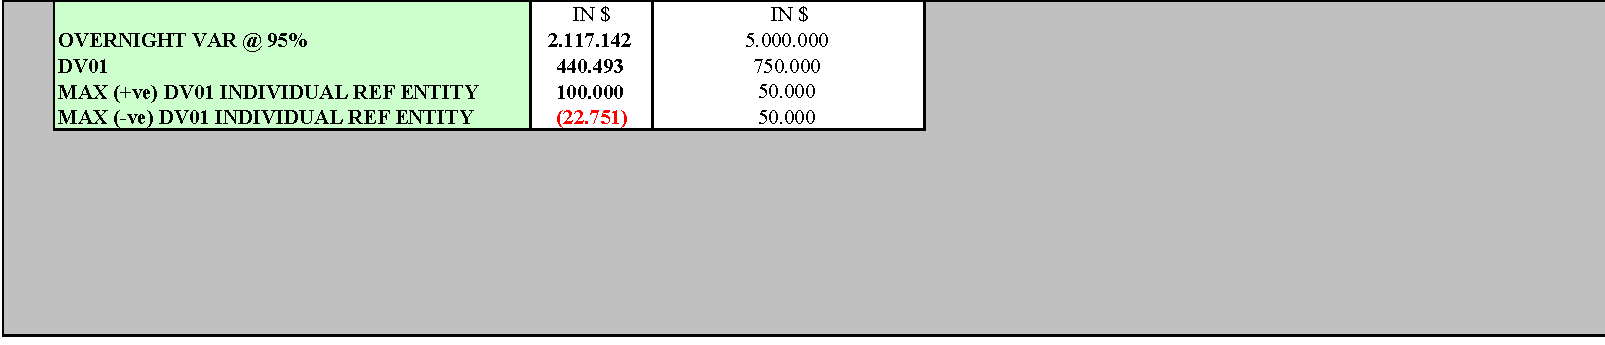
\includegraphics[width=0.323\textwidth]{evidence/xml-methods/native-vector/enron/Original.pdf} &
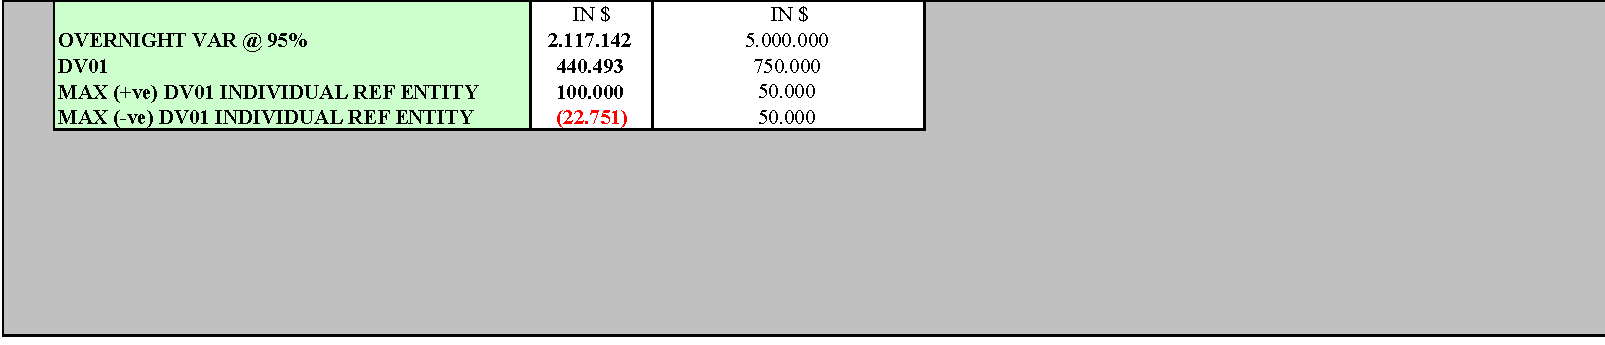
\includegraphics[width=0.323\textwidth]{evidence/xml-methods/native-vector/enron/Default.pdf} &
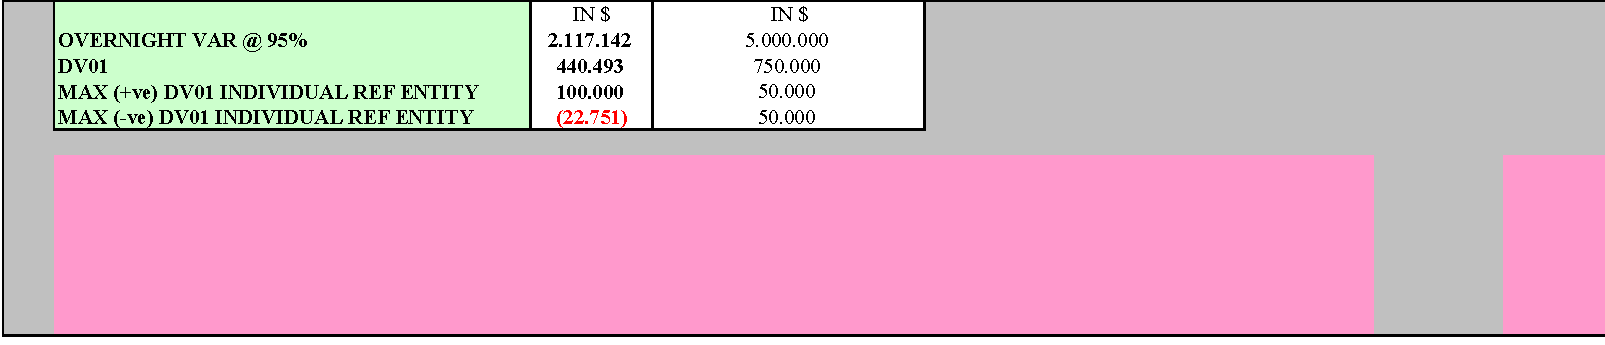
\includegraphics[width=0.323\textwidth]{evidence/xml-methods/native-vector/enron/Check-Performance.pdf}
\end{tabular}
\caption{An empty cell masks inherited formatting. In the Enron example, gray B31
overrides a pink column fill. SheetShrink preserves the mask; Check Performance
removes it and exposes pink. Native print exports match for Original and
SheetShrink after full rebuild within the displayed region. XML is abbreviated.}
\label{fig:fill-override-native}
\end{figure*}
